\section{Gateway}
\label{sec:app-gw}

Para a construção do \emph{Gateway} foi feita a instalação e configuração do
\emph{MQTT Broker} \emph{Mosquitto} em um dos RPI3.

\begin{citacao}

	Eclipse Mosquitto™ é um distribuidor de mensagens de código aberto (EPL/EDL
	licenciado) que implementa o protocolo MQTT versões 3.1 e 3.1.1. O MQTT
	fornece um método leve de transmitir mensagens usando um modelo de
	publicação/inscrição. Isso o torna adequado para mensagens "Internet das
	Coisas", como com sensores de baixa potência ou dispositivos móveis, como
	telefones, computadores embutidos ou microcontroladores como o Arduino. \

	\citeonline{mosquitto} Tradução Nossa.
\end{citacao}


A instalação é realizada com o gerenciador de pacotes \emph{apt-get} padrão do
\emph{raspbian} como mostrado na primeira linha da listagem abaixo.


\begin{lstlisting}[language=bash]
pi@broker:~ $ sudo apt-get install mosquitto
pi@broker:~ $ sudo sh -c 'echo "password_file /etc/mosquitto/passwd"
	>> /etc/mosquitto/mosquitto.conf'
pi@broker:~ $ sudo mosquitto_passwd -c /etc/mosquitto/passwd user
Password:
Reenter password:
pi@broker:~ $
\end{lstlisting}




\begin{figure}[htb]
\centering
	\begin{minipage}{0.32\textwidth}
	\centering
		\caption{\label{fig-ad-publish}MQTT Dashboard: Envio de mensagens}
		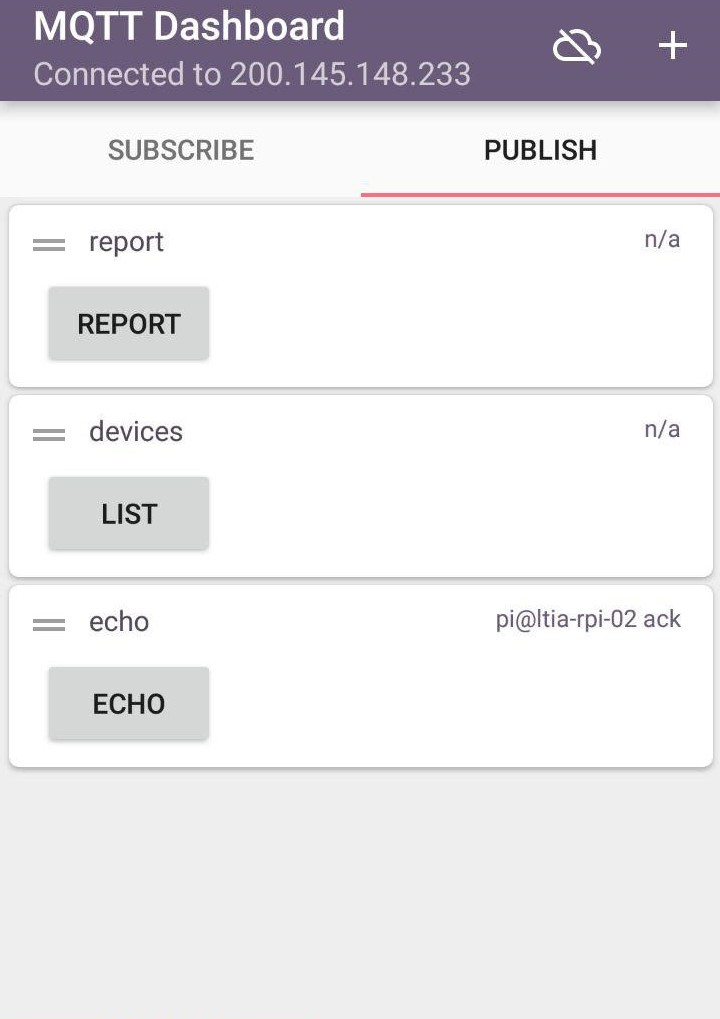
\includegraphics[width=1\textwidth]{052-gateway/mqtt/ad-publish.jpg}
		\legend{Fonte: Produzido pelo autor}
	\end{minipage}
\hfill
	\begin{minipage}{0.32\textwidth}
	\centering
		\caption{\label{fig-ad-home-ack}MQTT Dashboard: Lista de inscrições}
		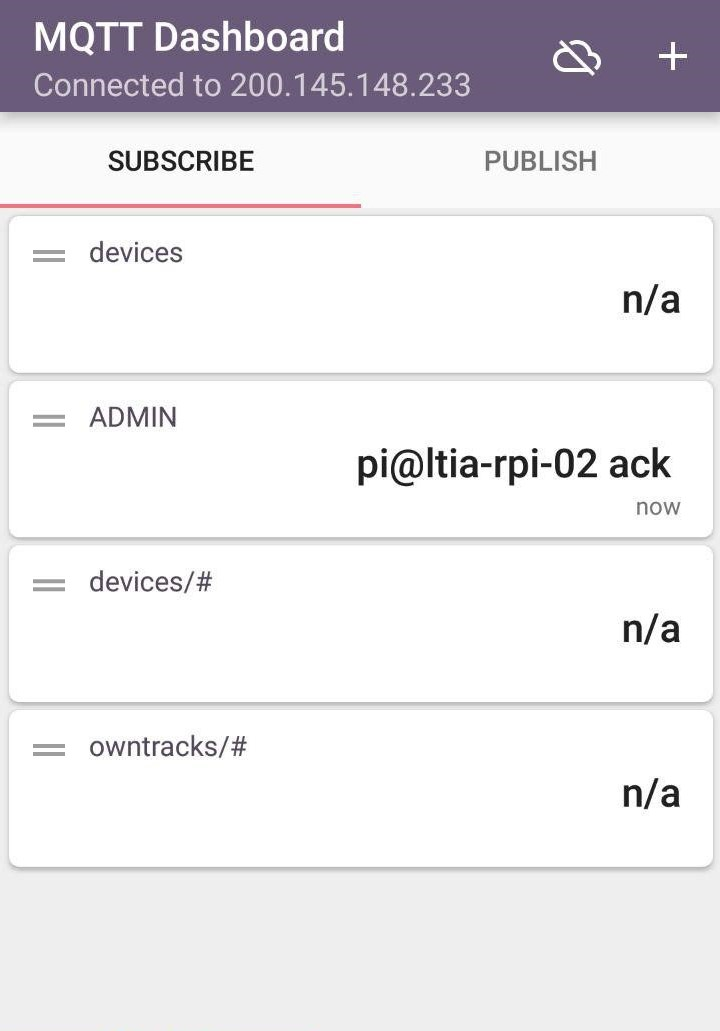
\includegraphics[width=1\textwidth]{052-gateway/mqtt/ad-home-ack.jpg}
		\legend{Fonte: Produzido pelo autor}
	\end{minipage}
\hfill
	\begin{minipage}{0.32\textwidth}
	\centering
		\caption{\label{fig-ad-admin-ack}MQTT Dashboard: Lista de mensagens no tópico}
		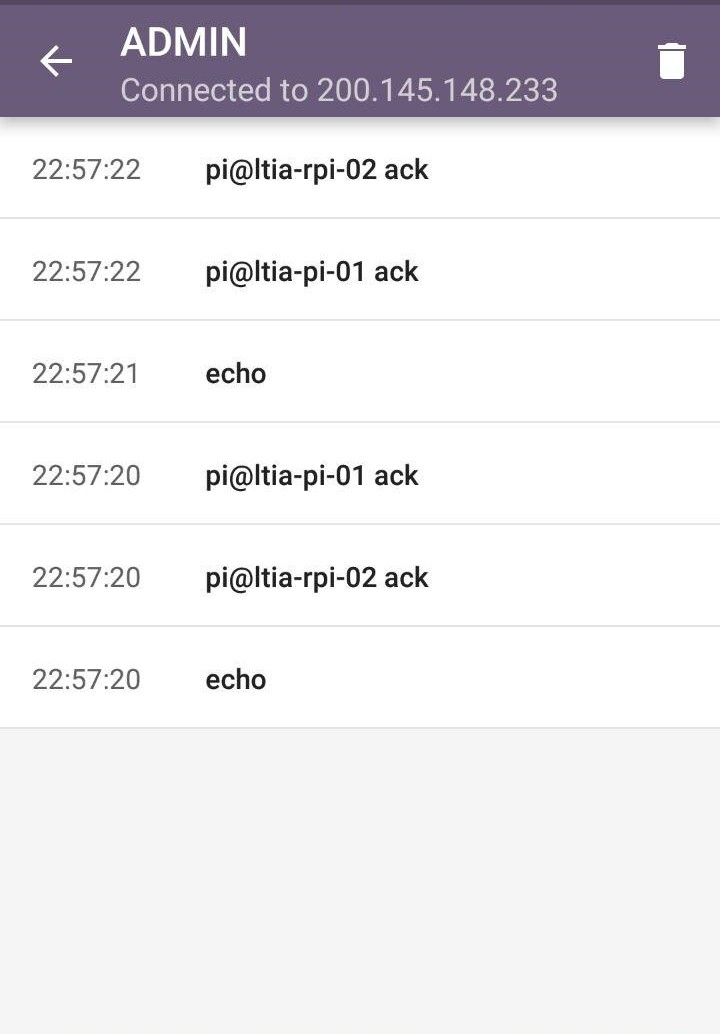
\includegraphics[width=1\textwidth]{052-gateway/mqtt/ad-admin-ack.jpg}
		\legend{Fonte: Produzido pelo autor}
	\end{minipage}
\end{figure}

\begin{figure}[htb]
	\begin{minipage}{0.49\textwidth}
		\centering
		\caption{\label{fig-mqttfx-stats}MQTT.fx: Estatísticas do \emph{Broker}}
		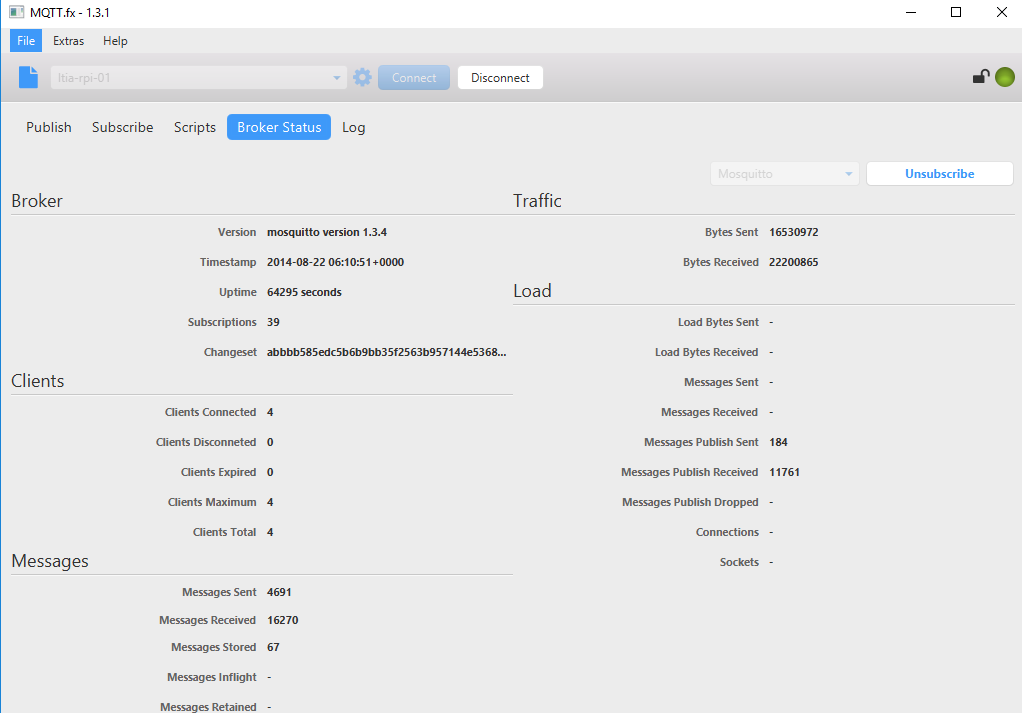
\includegraphics[width=1\textwidth]{052-gateway/mqtt/mqttfx-stats.png}
		\legend{Fonte: Produzido pelo autor}
	\end{minipage}
\hfill
	\begin{minipage}{0.49\textwidth}
		\centering
		\caption{\label{fig-mqtt-spy-list}mqtt-spy: Listagem de dispositivos}
		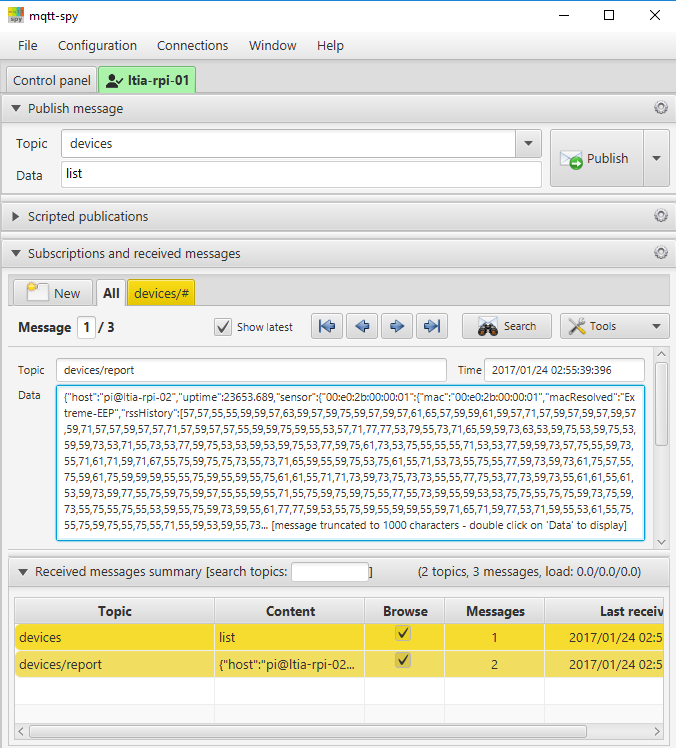
\includegraphics[width=1\textwidth]{052-gateway/mqtt/mqtt-spy-list.png}
		\legend{Fonte: Produzido pelo autor}
	\end{minipage}
\end{figure}
